\section{Zielsetzung}
In diesem Versuch wird die Halbwertszeit und die Zerfallskurve eines Isotops und eines istabilen Isotopengemische bestimmt.
Zur Bestimmung wird die Aktivierung mit Neutronen verwendet.
\section{Theorie}
\label{sec:Theorie}
Die Halbwertszeit $T$ beschreibt die Wahrscheinlichkeit des Zerfalls eines Nuklids.
Um die Halbwertszeit zu bestimmen werden Nuklide verwendet, dessen Halbwertszeit zwischen Sekunden und Stunden messbar sind.
Diese Nuklide entstehen, wenn ein stabiler Kern mit Neutronen beschossen wird.

\subsection{Kernreaktionen mit Neutronen}
Wird ein Kern mit einem Neutronen beschossen, wird dies vom Kern absorpiert.
Es entsteht ein neuer Kern A* der als Zwischkern oder Compoundkern bezeichnet wird.
Die aufgenommene Energie verteilt sich auf die Nukleonen.
Aufgrund dessen kommt es zur sogenannten Aufheizung des Zwischenkerns, da die Nukleonen einen höheren Energiezustand befinden.
Damit der der Zwischenkern wieder in den Grundzustand gelangt, werden $\gamma$-Quanten emittiert, da das aufgenommene Neutron nicht wieder abgestoßen werden kann.
\begin{equation}
    \ce{^{m}_{z}A} + \ce{^{1}_{0}n} -> \ce{^{m+1}_{z}A^*} -> \ce{^{m+1}_{z}A} + \gamma
\end{equation}
Der neue Kern ist instabil.
Damit der Kern stabil wird, wird ein Elektron emittiert.
Die Überschüssige Masse des neuen Kerns, wird in kinetische Energie von Elektronen umgewandelt.
\begin{equation}
    \ce{^{m+1}_{z}A} -> \ce{^{m+1}_{z+1} C} + \beta^- + E_\text{kin} +\nu_e
\end{equation}
Der Wirkungsquerschnitt $\sigma$ beschreibt die Wahrscheinlichkeit, dass der stabile Kern ein Neutron einfängt.
Dabei müsste der Kern eine bestimmte Fläche besitzten, damit dies möglich ist.
Für die Berechnung gilt 
\begin{equation}
    \sigma = \frac{u}{n K d}.
\end{equation}
Dabei beschreibt $d$ die Dicke einer Fläche einer Folie die Beispielsweise mit Neutronen bechossen werden, $K$ die Atome/$cm^3$, n Neutronen pro Sekunde und $u$ Einfängen. 
Die Einheit beträgt dabei $1 \unit{barn} \coloneq 10^{-24} \unit{\centi\meter\squared}$.
Über die Geschwindigkeit der Neutronen lässt sich die De-Broglie Wellenlänge $\lambda = h/m_n v$ berechnen.
Wenn die Wellenlänge $\lambda$ kleiner als der Radius ist, kann der Kern als Zielscheibe für dei Neutronen betrachtet werden.
Die Gesetzte der Optik für die Streuung des Lichtes an einem Objekt können analog betrachtet werden.
Wenn $R \leq \lambda$ gilt, sind die Neutronen langsamer.
Der Wirkungsquerschnitt eines Kerns, ist bei bestimmten Neutronengeschwindigkeiten um mehrere Zehnerpotenzen größer, als der Geometrische Querschnitt.
Wenn die die Differenz zweier Energieniveaus des Zwischenkerns glei der Energie des Neutrons ist, kommt es zur Resonanzabsoption.
Der Wirkungsquerschnitt ist somit proportional zu $1/v$.
Somit ist die Wahrscheinlichkeit für das Einfangen des Neutrons bei kleineren Geschwindigkeit der Neutronen größer, da diese sich länger in der Einwirkungssphäre des Kerns befindet.

\subsection{Erzeugung niederenrgetischer Neutronen}
Die Neutronen als freies Teilchen kommen in der Natur nicht vor, da sie einen instabielen Kern besitzten.
Aufgrunddessen müssen diese erzeugt werden.
Die Neutronen werden dafür mit $\ce{^{9} Be}$ Kernen und $\alpha$-Teilchen welche durch den Zerfall aus $\ce{^{266} Ra}$ entstehen beschossen.
Die Neutrinen haben dabei ein kontinuirliches Energiespektrum.
Damit die Neutronen abgebremst werde, wird eine Materieschicht verwendet, durch diese diffundieren.
Dabei stoßen die leichte Atomkerne mit den Neutronen elastisch zusammen, wodurch diese Energie an die Atomkerne abgibt.
Am geeignetsten lässt sich dafür Wasserstoff verwendet.
Die Neutronenquelle besitzt einen Mantel aus Paraffin. 
\begin{figure}
    \centering
    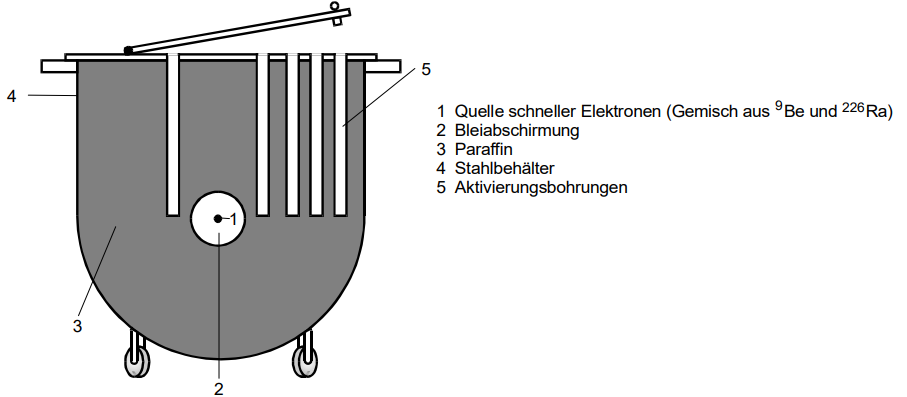
\includegraphics[scale=0.5]{content/Quelle Neutronen.png}
    \caption{Abbildung der verwendetetn Quelle für thermische Neutronen.}
    \label{fig:QN}
\end{figure}
Die Protonen des Paraffin und die Neutronen stoßen solange zusammen, bis die Nergie der mittleren kinetischen Energie der Moleküle liegt.
Diese liegt bei $\qty{0.025}{eV}$ bei einet Temperatur von $T= \qty{290}{K}$. 
Die Neutronen besitzten dann eine mittlere Geschwindigkeit von $2.2 km/sec$.
Diese Neutronen werden als thermische Neutronen bezeichnet.

\subsection{Untersuchung der Halbwertszeit}
Zu einem Zeitpunkt $t$ Anzahl an noch nicht zerfallenen Kerne $N(t)$ kann durch
\begin{equation}
    \label{eq:Nt}
    N(t) = N_0 e^{-\lambda t}
\end{equation}
bestimmt werden.
Dabei beschreibt $N_0$ die Anzahl instabieler Kerne zum Zeitpunkt $t = 0$ und $\lambda$ die Zerfallskonstante.
Durch den Zusammenhang der Halbwertszeit mit der Zerfallskonstante ergibt sich 
\begin{equation}
    \label{eq:T}
    T = \frac{\ln(2)}{\lambda}.
\end{equation}
Zur besseren Bestimmung der Anzahl zerfallener Kerne wird diese in einem festem Zeitintervall $\Delta t$ bestimmt.
Mithilfe eines geeigneten Strahlungsddetektor, kann jeder Zerfall durch Abgabe eines elektrischen Impulses gemessen werden.
Es liegt zwischen $N_{\Delta t}$ und der Zeit ein exponentieller Zusammenhang.
Somit kann $N_{\Delta t}$ berechnet werden aus
\begin{equation}
    N_{\Delta t}(t) = N(t) - N(t + \Delta t).
\end{equation}
Mit \ref{eq:NT} ergibt sich
\begin{equation}
    \ln N_{\Delta t}(t) = \ln N_0(1 - e^{-\lambda \Delta t}) -\lambda t,
\end{equation}
wobei $\ln N_0(1 - e^{-\lambda \Delta t})$ konstant ist.


\cite{sample}
